\documentclass[11pt]{article}
\usepackage{fullpage}
\usepackage{amsmath,amsthm,amssymb,amsfonts,multirow}
\usepackage{mathtools}
\usepackage{graphicx}
\usepackage{xcolor}
\usepackage{float}
%\usepackage{enumerate}
\usepackage[shortlabels, inline]{enumitem}
\usepackage{textcomp}
\usepackage{hyperref}
\usepackage{comment}

\usepackage{listings}
\lstset{language=Python, numbers=left, basicstyle=\ttfamily, keywordstyle=\color{blue}, showstringspaces=false}

\usepackage[style=alphabetic-verb]{biblatex}
% \bibliography{Problems/ref.bib}

\newcommand{\N}{\mathbb{N}}
\newcommand{\Z}{\mathbb{Z}}
\newcommand{\Q}{\mathbb{Q}}
\newcommand{\R}{\mathbb{R}}
\newcommand{\C}{\mathcal{C}}
\newcommand{\K}{\mathbb{K}}
\renewcommand{\div}{\mid}
\newcommand{\ndiv}{\nmid}
\newcommand{\E}{\mathbb{E}}
\newcommand{\I}{\mathbb{I}}
\newcommand{\F}{\mathcal{F}}

\DeclareMathOperator{\id}{Id}
\DeclareMathOperator{\tr}{Tr}
\DeclareMathOperator*{\argmax}{arg\,max}
\DeclareMathOperator{\lcm}{lcm}
\DeclareMathOperator{\spn}{span}
\DeclareMathOperator{\acosh}{acosh}

\DeclarePairedDelimiter{\floor}{\lfloor}{\rfloor}
\DeclarePairedDelimiter{\ceil}{\lceil}{\rceil}
\DeclarePairedDelimiter{\abs}{\lvert}{\rvert}

\newcommand{\subtag}[1]{\tag{\theparentequation#1}}

\renewcommand{\vec}[1]{\mathbf{#1}}

\usepackage{subfiles}
\usepackage{subcaption}
\makeatletter
\newcommand\nocaption{
    \renewcommand\p@subfigure{}
    \renewcommand{\thesubfigure}{\arabic{figure}\alph{subfigure}}
}
\makeatother


\newenvironment{problem}[2][Q]{\begin{trivlist}
\item[\hskip \labelsep {\bfseries #1}{\bfseries #2}]}{\end{trivlist}}

\newenvironment{solution}{%
  \begin{proof}[\textbf{Solution}]$ $\par\nobreak\ignorespaces
}{%
  \end{proof}
}

\theoremstyle{definition}
\newtheorem{definition}{Definition}
\newtheorem{theorem}{Theorem}
\newtheorem{lemma}{Lemma}

\hypersetup{
    colorlinks=true,
    linkcolor=blue,
    filecolor=magenta,      
    urlcolor=cyan,
    pdftitle={Overleaf Example},
    pdfpagemode=FullScreen,
    }


\title{Intro to Computational Mathematics: Section 7}
\date{October 2025}

\begin{document}
\maketitle

\begin{problem}{1. (True/False, 20pts)}
Only  state whether the statement is true or false (worth 5pts each).
\begin{enumerate}[(a)]
    \item For any real number $x > 0$ and differentiable, positive valued functions $f$ and $g$, the condition number of $f \circ g$ at $x$ is the condition number of $g$ at $x$ times the condition number of $f$ at $g(x)$
    \item For any overdetermined system of equations $Ax = b$, minimizing $\|Ax - b\|_2$ can be formulated as a square linear system via a related normal equation.
    \item The sequence $\epsilon_k = 1/k$ converges linearly to zero.
    \item If Newton's method is initialized sufficiently close to the root of a nonlinear equation $f(x) = 0$, it will eventually converge to that root.
\end{enumerate}
\end{problem}
\begin{solution}
\begin{enumerate}[(a)]
\item This is true. To see this: observe that:
    \begin{align*}
        \kappa_{(f \circ g)}(x) &= \abs*{\frac{x (f \circ g)'(x)}{(f \circ g)(x)}} \\
        &= \abs*{\frac{x f'(g(x))g'(x)}{f(g(x))}} \\
        &= \abs*{\frac{x f'(g(x))g'(x)}{f(g(x))} \cdot \frac{g(x)}{g(x)}} \\
        &= \abs*{\frac{g(x)f'(g(x))}{f(g(x))} \cdot \frac{xg'(x)}{g(x)}} \\
        &= \abs*{\frac{yf'(y)}{f(y)} \cdot \frac{xg'(x)}{g(x)}} \\
        &= \abs*{\frac{yf'(y)}{f(y)}} \cdot \abs*{\frac{xg'(x)}{g(x)}} \\
        &= \kappa_f(g(x)) \cdot \kappa_g(x)
    \end{align*}
\item This is true. The normal equations for an overdetermined linear system are given by $$A^TAx = A^T b.$$ Notice that $A^TA$ is always a square matrix.
\item This is false. In order for the sequence to converge linearly, we would need $$\lim_{k \rightarrow \infty}\abs*{\frac{\epsilon_{k+1}}{\epsilon_k}} \eqqcolon \sigma < 1.$$ However, $$\lim_{k \rightarrow \infty}\abs*{\frac{\epsilon_{k+1}}{\epsilon_k}} = \lim_{k \rightarrow \infty}\abs*{\frac{1/(k+1)}{(1/k)}} = \lim_{k \rightarrow \infty}\abs*{\frac{k}{k+1}} = 1 \nless 1.$$
\item This is false. Newton's method requires differentiability in order to guarantee convergence. Consider the function $f(x) = \begin{cases}0 \qquad x = 0 \\ 1 \qquad \text{otherwise}\end{cases}$. This function has derivative 0 for any point near the root, so Newton's method will never change values at any step of iteration and will never converge to the root.
\end{enumerate}
\end{solution}
\newpage



\begin{problem}{2. (Stability of Some Computations, 30pts)}
Consider the function $f, g: \R \rightarrow \R$:
$$\begin{cases}
    f(x) = \frac{x-1}{x^2-1} \\
    g(x) = \frac{1}{x+1}.
\end{cases}$$
These two functions are actually equal (that is, for all $x \in \R$, $f(x) = g(x)$)! Despite this, the implementations below evaluate to different values at $1 - 10^{-9} = 0.999999999$.
\begin{center}
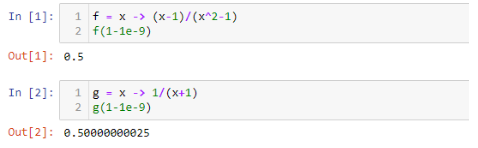
\includegraphics[width=0.8\textwidth]{question2_fig.png}
\end{center}
\begin{enumerate}[(a)]
    \item (10pts) Compute formulas for the condition numbers $\kappa_f(x)$ and $\kappa_g(x)$ wherever they are well-defined.
    \item (10pts) Consider now the potential inaccuracies introduced by each individual step needed to implement the computation of $f(x)$ on a standard IEEE (64bit) computer. Based on the conditioning of each underlying step, approximately to how many digits should we trust the above estimate of $f(1 - 10^{-9}) \approx 0.5$?
    \item (10pts) Similarly, consider now the potential inaccuracies by each individual step needed to implement the computation of $g(x)$ on a standard IEEE (64bit) computer. Based on the conditioning of each underlying step, approximately to how many digits should we trust the above estimate of $g(1 - 10^{-9}) \approx 0.50000000025$?
\end{enumerate}
\end{problem}
\begin{solution}
\begin{enumerate}[(a)]
\item \begin{tabular}{c|c}
    $f(x)$ & $\kappa$ \\\hline
    $x_1 = x - 1$ & $\frac{1 - 10^{-9}}{10^{-9}} \approx 10^9$ \\
    $x_2 = x^2$ & 2 \\
    $x_3 = x_2 - 1$ & $\abs*{\frac{1 - 2(10^{-9}) + 10^{-18}}{-2(10^{-9}) + 10^{-18}}} \approx 0.5(10^{9})$ \\
    $x_4 = x_1/x_3$ & $1$
\end{tabular}
\begin{tabular}{c|c}
    $g(x)$ & $\kappa$ \\\hline
    $x_1 = x + 1$ & $\frac{1 - 10^{-9}}{2 - 10^{-9}} \approx 1/2$ \\
    $x_2 = 1/x_1$ & $1$
\end{tabular}
\item Since the computation of $x_4$ total divides approximately equivalent digits of precision, we lose approximately 9 digits of precision in computing $f$, so we should expect accuracy up to about $16 - 18 = 7$ digits.
\item For computing $g$, no step in the computation really loses accuracy, so we can expect to trust all $16$ digits of precision.
\end{enumerate}
\end{solution}
\newpage



\begin{problem}{3. ($LU$ factorizations and Subtractive Cancellations by Hand, 20pts)} (5pts) Determine whether or not the matrix below is an orthogonal matrix.
$$A = \begin{bmatrix*}1/2 & -1/2 \\ 1/2 & 1/2\end{bmatrix*}$$

(15pts) Compute an $LU$ factorization of the matrix $A$ above and then doing forward/backward substitutions to solve the system $Ax = b$ with $b = \begin{bmatrix*}10^{-12} \\ 1\end{bmatrix*}$.

Clearly state the matrices $L, U$ and vectors $z, x$ you compute. If a bad subtractive cancellation would occur during your arithmetic if done on a computer in floating point, clearly label it.
\end{problem}
\begin{solution}
\begin{align*}
    A^T A &= \begin{bmatrix*}1/2 & -1/2 \\ 1/2 & 1/2\end{bmatrix*}^T \begin{bmatrix*}1/2 & -1/2 \\ 1/2 & 1/2\end{bmatrix*} \\
    &= \begin{bmatrix*}1/2 & 1/2 \\ -1/2 & 1/2\end{bmatrix*} \begin{bmatrix*}1/2 & -1/2 \\ 1/2 & 1/2\end{bmatrix*} \\
    &= \begin{bmatrix*}1/2  & 0 \\ 0 & 1/2 \end{bmatrix*}
\end{align*}
so $A$ is not orthogonal.

For the $LU$ decomposition, we start by taking the first row of $A$ for $U$. $U_{(1, :)} = \begin{bmatrix*}1/2 & -1/2\end{bmatrix*}$ and compute the first column of $L$ accordingly: $L_{(:, 1)} = \begin{bmatrix*}1 \\ 1\end{bmatrix*}$. Subtracting $A - L_{(:, 1)} U_{(1, :)} = \begin{bmatrix*}
    0 & 0 \\ 0 & 1
\end{bmatrix*}$. We finish the decomposition with the last row as:

$L = \begin{bmatrix*}
    1 & 0 \\
    1 & 1
\end{bmatrix*}$, $U = \begin{bmatrix*}
    1/2 & -1/2 \\ 0 & 1
\end{bmatrix*}$

Now letting $z = Ux$, we compute $Lz = b$ using forward substitution $z = \begin{bmatrix*}
    10^{-12} \\
    \frac{1 - 10^{-12}}{1}
\end{bmatrix*}$. Lastly, via back-substitution, we solve $Ux = z$ as: $x = \begin{bmatrix*}
    (-1/2)(1 - 10^{-12})/(1/2)\\
    10^{-12}
\end{bmatrix*} = \begin{bmatrix*}
    10^{-12} - 1 \\ 10^{-12}
\end{bmatrix*}$ with no bad subtractive cancellations.
\end{solution}
\newpage



\begin{problem}{4. (Polynomial Rootfinding, 30pts)}
Consider a degree five polynomial $f$ with all real roots where every root lies between $0$ and $10$. As an example, consider $$f(x) = x^5 - 14x^4 + 75x^3 - 190x^2 + 224x - 96$$ which has four roots occurring at $x = 1, 2, 3, 4$ and no others.
\begin{enumerate}[(a)]
    \item (15pts) The professor ran three different rootfinding methods on the example $f$ above initialized at zero. The first five iterates $x_k$ as these methods are given below, truncated to display to an absolute accuracy of only $10^{-7}$. For each method,
    \begin{enumerate}[(i)]
        \item Describe the kind of convergence (or lack thereof) that appears to be occurring.
        \item Estimate at what iteration $k$ will first have $x_k$ within machine precision of a root at $f$.
    \end{enumerate}
    \begin{tabular}{c|c|c|c}
        & Method 1 & Method 2 & Method 3 \\\hline
        $x_0$ & 0 & 0 & 0 \\
        $x_1$ & 0.5127243 & 1.8436643 & 7.6559001 \\
        $x_2$ & 0.8436351 & -2.1934825 & 4.5004557 \\
        $x_3$ & 0.9215462 & 3.4734588 & 2.9615434 \\
        $x_4$ & 0.9634797 & -6.7342356 & 3.0003454 \\
        $x_5$ & 0.9813022 & 12.8435311 & 2.9999998
    \end{tabular}
    \item (15pts) The above rootfinding methods together seem to have only identified two roots of $f$. In particular, they found $x = 1$ and $x = 3$ are roots of $f$. Propose a reliable algorithm that will efficiently compute every root of any such polynomial $f$ to high precision. You can use any method discussed in class as a subroutine without specifying its particular details.
\end{enumerate}
\end{problem}
\begin{solution}
\begin{enumerate}[(a)]
    \item We start with method 2 as this sequence is clearly not converging. To describe the convergence of methods 1 and 3 we first write down an approximation of the errors at each step (to the nearest root at the convergence point).
    
    \begin{tabular}{c|c|c}
        & Method 1 & Method 3 \\\hline
        $\epsilon_0$ & 1 & 3 \\
        $\epsilon_1$ & 0.49 & 4.65 \\
        $\epsilon_2$ & 0.16 & 1.50 \\
        $\epsilon_3$ & 0.08 & 0.04 \\
        $\epsilon_4$ & 0.04 & 0.0003 \\
        $\epsilon_5$ & 0.02 & 0.0000002
    \end{tabular}
    
    For method 1, relative error $\frac{\epsilon_{k+1}}{\epsilon_k}$ appears to be approximately 1/2 every time and so see linear convergence. Each step we gain approximately one bit of accuracy, so we should expect $k = 52$ to have machine precision of a root of $f$.
    
    Method 3 appears to have quadratic convergence as the number of zeros doubles towards the later steps. Each step we double the number of accurate bits and so we should expect about $\log_2(52) \approx 6$ steps after the error is smaller than $1$ before we seen machine precision. Thus $k = 9$ seems reasonable to expect machine precision on the root.
    \item One method for finding all roots of a polynomial is to simply find a root $r(f)$ and then remove it from the polynomial by dividing $f$ by the monomial term $(x - r(f))$. In this way we build a sequence of decreasing degree polynomials $f^{(0)}, f^{(1)}, \ldots, f^{(n)}$. In order to find a root of $f^{(k)}$ we can use Newton's method for approximately 10 steps (since it will have quadratic convergence on polynomials).
    
    Well this will work, it is likely to cause numerical instability in practice as each root found will have some error. In order to refine this approach, we can call the root found by Newton's method on $f^{(k)}$ to be a candidate root. We will refine the candidate root by taking another 10 steps of Newton's method on $f = f^{(0)}$ starting with the candidate root. This way we will find each root of $f$ within machine precision and lose less accuracy in the iteration.

    Since we are assuming the domain of the roots is bounded, we can use other techniques to first bound the domains of each root (e.g. using Intermediate Value Theorem and/or Decartes' Rule of Signs) and then search for each successive root within the bounded region.
\end{enumerate}
\end{solution}



\end{document}
